\documentclass[aspectratio=169]{beamer}

%---------------------------
%       Beamer Cheat Sheet
%---------------------------
% https://www.cpt.univ-mrs.fr/~masson/latex/Beamer-appearance-cheat-sheet.pdf

%---------------------------
%       Set Theme and Colors
%---------------------------

\usetheme[width=.1\paperwidth]{Hannover}
% \setbeamertemplate{sidebar canvas right}[vertical shading][top=red,bottom=blue]

\definecolor{QESblue}{HTML}{8AD2ED}
\definecolor{QESdarkblue}{HTML}{187ca2}
\definecolor{QESlightblue}{HTML}{c4e8f6}

\setbeamercolor{sidebar}{bg=QESlightblue}
\setbeamercolor{titlelike}{fg=QESdarkblue}

\setbeamercolor{palette sidebar secondary}{fg=QESdarkblue}
\setbeamercolor{title in sidebar}{fg=QESdarkblue}
\setbeamercolor{author in sidebar}{fg=QESdarkblue}

\addtobeamertemplate{sidebar left}{}{\vfill \hspace{.006\paperwidth} 
\includegraphics[width=.08\paperwidth]{../../../logo.png} \vspace{.006\paperwidth} } 
% \addtobeamertemplate{sidebar left}{}{\vfill \hspace{.00001\paperwidth} 
\includegraphics[width=.093\paperwidth]{../../figures/qes-qr.png} \vspace{.003\paperwidth} } 

%---------------------------
%       No navigation symbols
%---------------------------
\setbeamertemplate{navigation symbols}{}

%---------------------------
%       Set Fonts
%---------------------------
\usepackage{helvet}
\renewcommand{\familydefault}{\sfdefault}
\usepackage{sansmathfonts}
\usepackage{upgreek}

\setbeamerfont{frametitle}{series=\bfseries, size=\Large}
\setbeamerfont{title in sidebar}{series=\bfseries, size=\small}
\setbeamertemplate{caption}{\it\raggedright\insertcaption\par}

%---------------------------
%       Math font packages
%---------------------------
\usepackage{dsfont, amsmath, amsthm, mathtools}
\usepackage{bbm, bm}
\usepackage[T1]{fontenc}
\usepackage[version=3]{mhchem}

%---------------------------
%       Figure packages
%---------------------------
\usepackage{graphicx}
\graphicspath{{../../figures}}

\usepackage{epstopdf}
\usepackage{color}

\setbeamerfont{caption}{size=\footnotesize}

\usepackage{subfigure}

%---------------------------
%       Manual placement packages
%---------------------------
\usepackage{tikz}
\usetikzlibrary{calc}

%---------------------------
%       Local Macros
%---------------------------

\newcommand{\manualpic}[4]{
    % inputs {filename}{figure options}{x offset}{y offset}
    \tikz[remember picture, overlay] \node[anchor=center] at ($(current page.center)+(#3,#4)$) {\includegraphics[#2]{#1}};
}

\newcommand{\manualtext}[3]{
    % inputs {text}{x offset}{y offset}
    \tikz[remember picture, overlay] \node[anchor=center] at ($(current page.center)+(#2,#3)$) {#1};
}

\newcommand{\manualtextleft}[3]{
    % inputs {text}{x offset}{y offset}
    \tikz[remember picture, overlay] \node[anchor=west] at ($(current page.center)+(#2,#3)$) {#1};
}

\newcommand{\manualtextright}[3]{
    % inputs {text}{x offset}{y offset}
    \tikz[remember picture, overlay] \node[anchor=east] at ($(current page.center)+(#2,#3)$) {#1};
}

\newcommand{\slidereference}[1]{
    \manualtextleft{\tiny #1}{-0.47\linewidth}{-0.47\textheight}
}

\newcommand{\dv}[2]{\frac{\mathrm{d}#1}{\mathrm{d}#2}}

\title{Ocean Carbon}
\author{1/5}

\begin{document}

\begin{frame}{How much carbon is in the ocean?}
    \textbf{Oscar Branson} \\ 
    \bigskip
    \href{mailto:ob266@cam.ac.uk}{ob266@cam.ac.uk} \\
    Earth Sciences \\
    Office M25
\end{frame}

\begin{frame}{Next five lectures...}

\textbf{Lectures}: Carbon in the ocean and the processes affecting it.

\begin{itemize}
    \item Concepts, turning concepts into equations. 
    \item Maths note: these equations will get too complex to solve analytically, we will be algebra \textsuperscript{LIGHT}.
\end{itemize}

\bigskip

\textbf{Practicals}: Modelling carbon in the ocean.

\begin{itemize}
    \item Will parallel lectures
    \item Coding up equations in lectures to make a model of carbon in the ocean.
\end{itemize}

\end{frame}

\section{Measurement}

\begin{frame}{Measuring Ocean Carbon}
    \centering

    \includegraphics<1>[width=\linewidth, totalheight=0.7\textheight, keepaspectratio]{carbon-GLODAP-map.jpg}
    \only<1>{
        \manualtext{\textbf{GLODAP}}{0.48\linewidth}{-0.3\textheight}
        \manualtext{1085 Cruises}{0.48\linewidth}{-0.35\textheight}
        \manualtext{1.4M samples}{0.48\linewidth}{-0.4\textheight}
        \slidereference{https://www.digitalearthviewer-glodap.geomar.de/}
    }    

    \includegraphics<2>[width=\linewidth, totalheight=0.75\textheight, keepaspectratio]{carbon-VINDTA.jpg}

    \includegraphics<3->[width=\linewidth, totalheight=0.75\textheight, keepaspectratio]{carbon-cx-dic.png}
    \only<3->{
        \manualtext{\rotatebox{90}{$\mathrm{\upmu mol~kg^{-1}}$}}{0.52\linewidth}{-0.6}
        \slidereference{Sarmiento \& Gruber (2006)}
    }

    \only<4>{
        \manualtextright{Average $\sim 2255~ \mathrm{\upmu mol~kg^{-1}}$}{0.5\linewidth}{-0.45\textheight}
    }

\end{frame}

\section{Inventory}

\begin{frame}{Ocean \& Atmosphere}

    \centering
    \includegraphics<1>[width=\linewidth, totalheight=0.75\textheight, keepaspectratio]{carbon-1box.png}

    \only<1>{
        \manualtext{71\% of Earth SA}{0.34\linewidth}{-0.22\textheight}
        \manualtext{3.7 km deep}{0.34\linewidth}{-0.27\textheight}
        \manualtext{$1.4 \times 10^{21}~kg$}{0.34\linewidth}{-0.32\textheight}
    }

\end{frame}

\section{Solubility}

\begin{frame}{Henry's Law}
    \ce{CO2} behaves as an \textbf{ideal gas}, and dissolves into water according to \textbf{Henry's Law}, which states that the concentration ($C$) of a gas dissolved in a liquid is proportional to the partial pressure ($P$) of the gas above the liquid:

    $$
    C = k P
    $$

    For \ce{CO2}, we write:

    $$
    \ce{[CO2]} = K_0\ \ce{pCO_2}
    $$

    \vfill
    \small \emph{(square brackets denote concentration in $\mu mol~kg^{-1}$)}

    \only<2>{
        \manualpic{carbon-janco2.png}{width=4cm}{5.5cm}{-1.5cm}
    }

\end{frame}

\section{Equilibrium?}

\begin{frame}{Equilibrium?}
    \centering
    \includegraphics<1>[width=\linewidth, totalheight=0.75\textheight, keepaspectratio]{carbon-1box.png}

    \includegraphics<2>[width=\linewidth, totalheight=0.75\textheight, keepaspectratio]{carbon-cx-dic.png}
    \only<2>{
        \manualtext{\rotatebox{90}{$\mathrm{\upmu mol~kg^{-1}}$}}{0.52\linewidth}{-0.6}
        \slidereference{Sarmiento \& Gruber (2006)}
    }

    \includegraphics<3>[width=\linewidth, totalheight=0.75\textheight, keepaspectratio]{carbon-ocean-atmos.png}
    \only<3>{
        \slidereference{Sarmiento \& Gruber (2006)}
    }

\end{frame}

\begin{frame}{Disequilibrium?}
    The atmosphere is not in equilibrium with the \textbf{average} ocean.

    \begin{itemize}
        \item<2-> \textbf{The ocean has structure} - it circulates and is stratified. Only the surface ocean equilibrates with the atmosphere.
        \item<3-> \textbf{\ce{CO2} reacts with water} to form non-exchangeable species, greatly increasing carbon concentration in water [L36].
        \item<4-> \textbf{Biological processes} take up carbon in the surface and export it into the deep ocean. [L37 \& L38]
    \end{itemize}
    
\end{frame}

\section{Sructure}

\begin{frame}{Ocean Structure}
    \centering
    
    \includegraphics<1>[width=\linewidth, totalheight=0.75\textheight, keepaspectratio]{carbon-cx-dic.png}
    \only<1>{
        \manualtext{\rotatebox{90}{$\mathrm{\upmu mol~kg^{-1}}$}}{0.52\linewidth}{-0.6}
        \slidereference{Sarmiento \& Gruber (2006)}
    }

    \includegraphics<2>[width=\linewidth, totalheight=0.8\textheight, keepaspectratio]{carbon-components.png}

    \includegraphics<3>[width=\linewidth, totalheight=0.75\textheight, keepaspectratio]{ocean-circulation.png}

    \includegraphics<4>[width=\linewidth, totalheight=0.75\textheight, keepaspectratio]{marshall-speer.png}


\end{frame}

\section{Modelling Ocean Carbon}

\begin{frame}{Modelling Ocean Carbon}
    \centering

    \only<1>{
        In \textbf{Practicals 13-16} you will be making a model of carbon in the ocean. \\
        ~ \\
        \Large \textbf{How should we approach this?}
    }

    \includegraphics<2>[width=0.8\linewidth, totalheight=0.75\textheight, keepaspectratio]{stommel_box.png}

    \includegraphics<3>[width=\linewidth, totalheight=0.75\textheight, keepaspectratio]{ocean-circulation.png}

\end{frame}

\begin{frame}{Simplification}

    \centering
    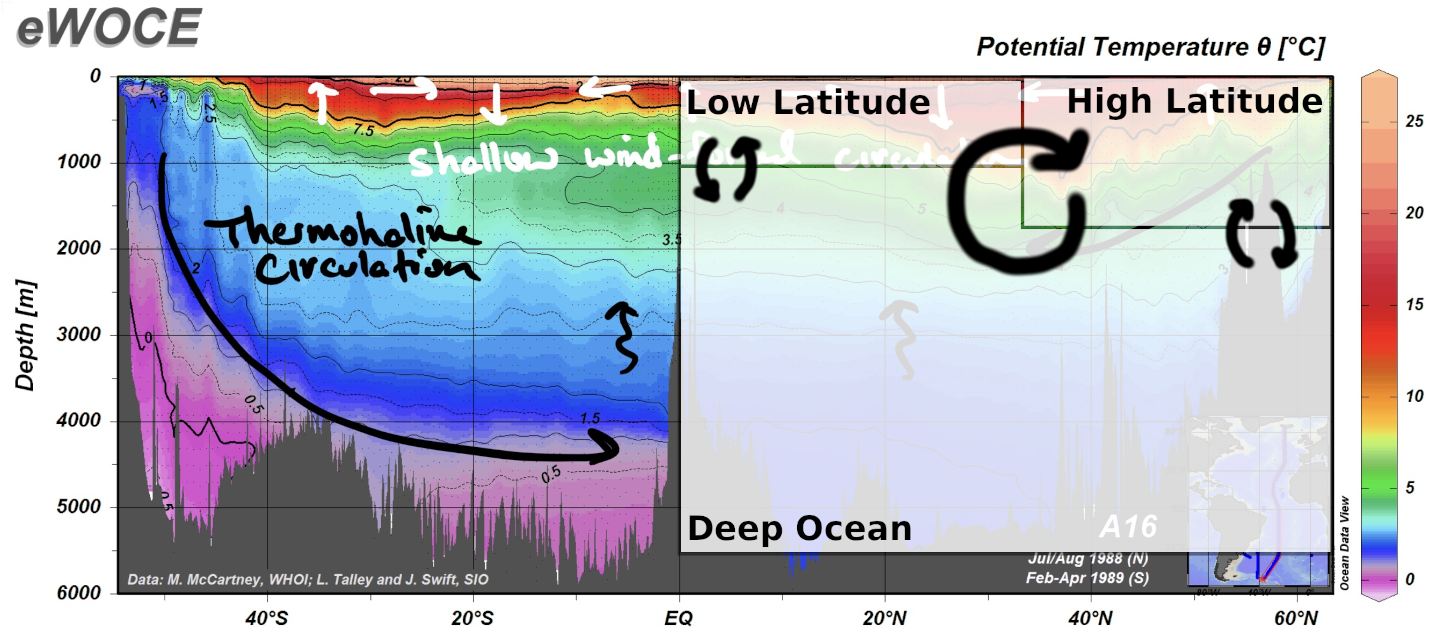
\includegraphics[width=\linewidth, totalheight=0.75\textheight, keepaspectratio]{ocean-circulation-annotated.png}

\end{frame}

\begin{frame}{3-Box Model}
    \begin{columns}
        \begin{column}{0.6\linewidth}
            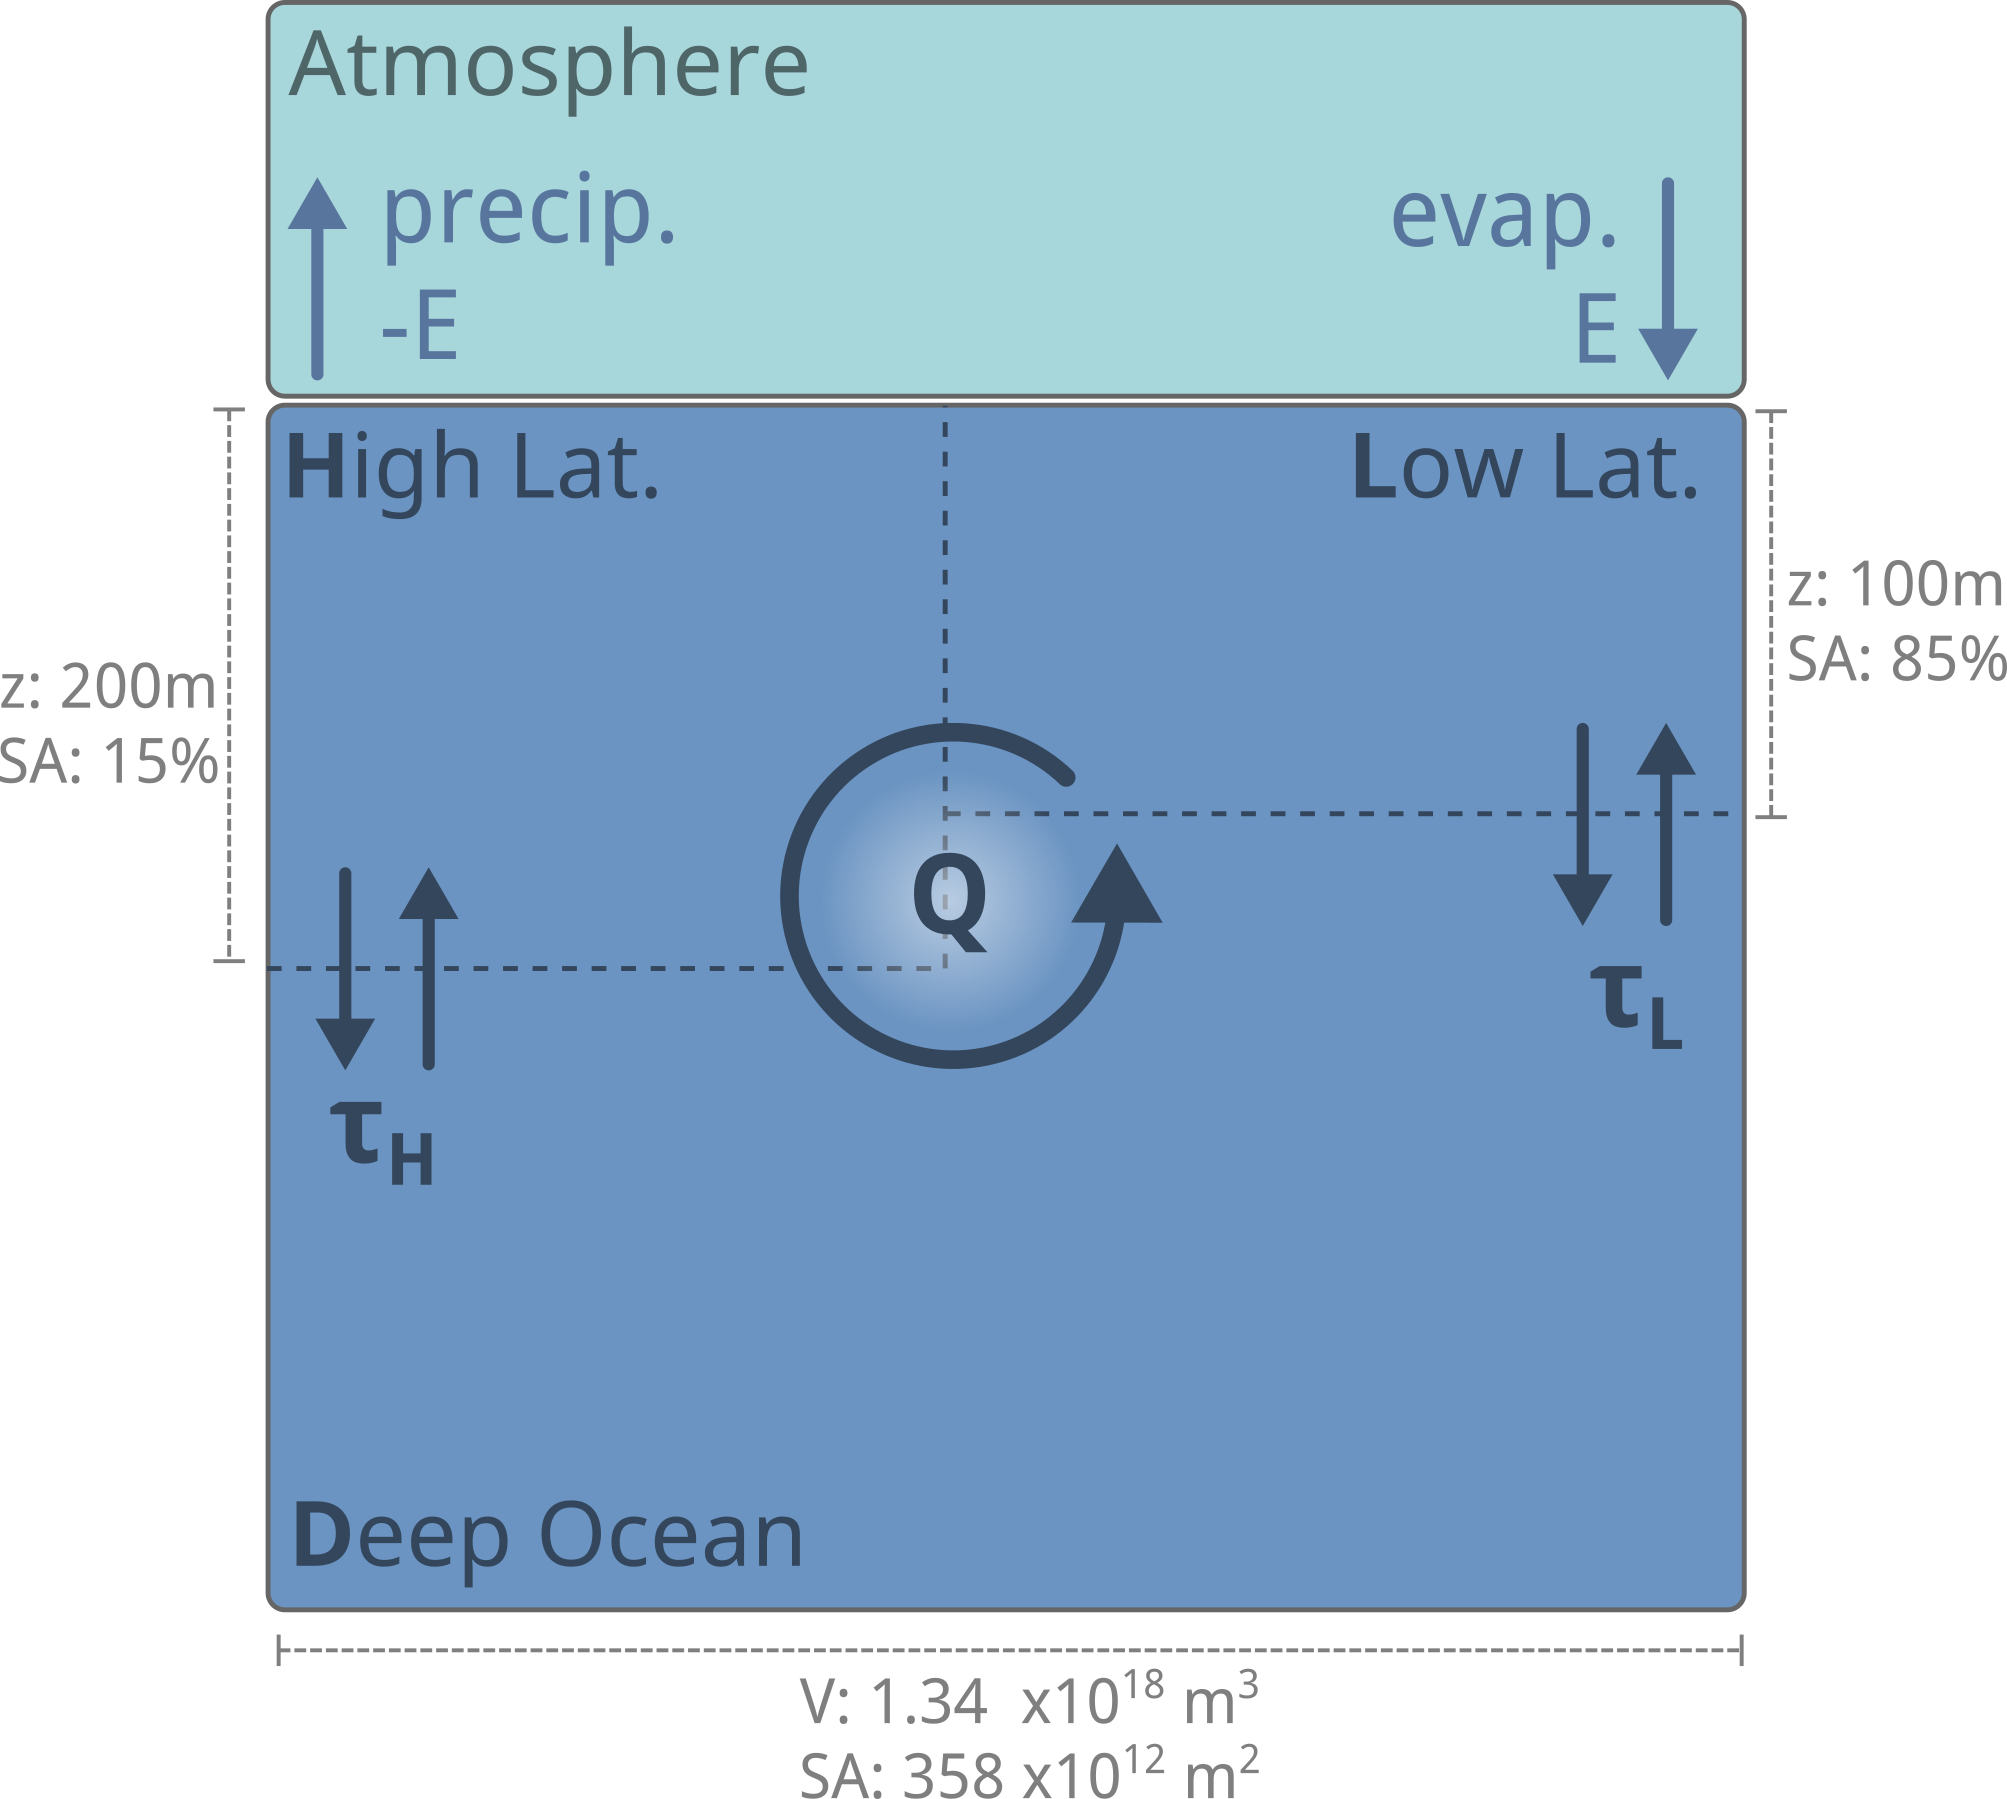
\includegraphics[width=\linewidth, totalheight=0.8\textheight, keepaspectratio]{ocean-3box.png}
        \end{column}   
        \begin{column}{0.3\linewidth}
            You will begin building this model in Practical 13.
        \end{column} 
    \end{columns}
    

\end{frame}

\begin{frame}{Conservative Transport}
    A \textbf{conservative} quantity is neither created nor destroyed. The total amount in the system remains constant, although model processes can partition it unevenly between boxes. For our model:
    \begin{align*}
    \dv{C_L}{t} &= \frac{q}{V_L} (C_D - C_L) - \frac{1}{\tau^{mix}_L} ( C_L - C_D ) \\
    \dv{C_H}{t} &= \frac{q}{V_H} (C_L - C_H) - \frac{1}{\tau^{mix}_H} ( C_H - C_D ) \\
    \dv{C_D}{t} &= \frac{q}{V_D} (C_H - C_D) +  \left. \left( \frac{V_L}{\tau^{mix}_L} ( C_L - C_D ) + \frac{V_H}{\tau^{mix}_H} ( C_H - C_D ) \right) \middle/ V_D \right.
    \end{align*}
\end{frame}

\begin{frame}{Temperature \& Salinity}
    \centering
    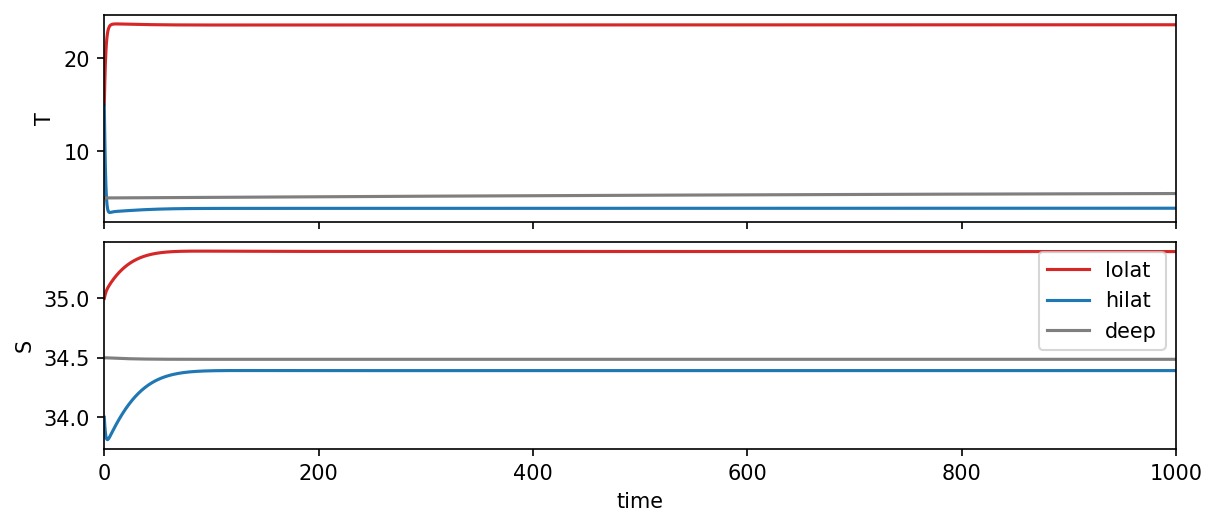
\includegraphics[width=\linewidth, totalheight=0.75\textheight, keepaspectratio]{carbon-model-TS.png}
\end{frame}

\section{Global Context}

\begin{frame}{Modern Carbon Cycle}
    \centering

    \includegraphics<1>[width=\linewidth, totalheight=0.85\textheight, keepaspectratio]{ipcc-carbon-cycle.jpg}
    \slidereference{IPCC AR5, Chapter 6}

\end{frame}

\end{document}


% \begin{frame}{TITLE}
% \end{frame}